\chapter{Definição e Preparação dos Estudos}

\label{cap-metodologia}
Este capítulo aborda o planejamento para a execução do projeto,
contendo os procedimentos e técnicas utilizados, a fim de
explicar como o desenvolvimento foi realizado para atingir os seus objetivos,
servindo como base para a sua reprodução em trabalhos futuros.

O trabalho é fundamentado na proposta de uma solução, utilizando conceitos e práticas
da engenharia de software, com a definição de um objetivo, a definição de um planejamento,
e a execução das atividades planejadas, e posteriormente a validação dos resultados. 
A principal contribuição deste trabalho está em ajudar a responder a seguinte questão:

\begin{center}
 \textbf{QP:}
  \textit{
  Como implantar aplicações web em sistema Debian GNU/Linux de forma automatizada e
  segura?
}
\end{center}

Dado objetivo e a questão problema, este trabalho consiste em contribuir
com a proposta de uma solução de gerência de configuração de software, que permita implantar
aplicações web em sistemas Debian GNU/Linux de forma automatizada e segura.

Além disso, a solução proposta deverá passar
por uma validação dos resultados, baseada na observação
da execução da solução em exemplos de uso. Cada exemplo conterá uma aplicação
real que deverá ser implantada com sucesso. Essa validação tem seus procedimentos
definidos na Seção \ref{subsection:validacao} e as definições dos exemplos de uso
estão na Seção \ref{subsection:exemplos}.

Inicialmente, foi realizada uma pesquisa dos trabalhos relacionados para compreender
quais eram as soluções na engenharia de software que buscam a automação da implantação
de aplicações web, a pesquisa tem como objetivo
gerar conhecimentos para aplicação prática,
relacionada a aplicações que auxiliam na implantação automatizada de software.

Os trabalhos encontrados serviram de insumo para auxiliar na construção do trabalho, 
a partir da análise dos resultados que foram encontrados. 

\section{Trabalhos Relacionados}
\label{section:trabalhos_relacionados}

Para compreender o que acontece na área relacionada com a implantação
automatizada de aplicações, foi feito uma busca de alguns trabalhos relacionados 
recentes. \citeonline{leo2014} em seu mestrado,
desenvolveu um sistema de middleware chamado CHOReOS Enactment Engine, que possibilita a implantação distribuída e automatizada de composições
de serviços web numa estrutura virtualizada, no qual opera no modelo
computacional conhecido como plataforma como serviço. Seu foco é na automação da 
implantação aliado com a gerência de recursos de 
hardware.

Existem ferramentas disponíveis no mercado que também trazem a proposta
de automação de instalação de aplicações, BitNami \footnote{https://bitnami.com/} é uma 
biblioteca de aplicativos populares e ambientes de desenvolvimento, 
que podem ser instalados com apenas um clique, 
através de uma interface web amigável. Ela automatiza todo o processo de 
compilar e configurar os aplicativos, 
e todas as suas dependências (bibliotecas de terceiros, linguagem de programação, 
bases de dados) para que o usuário comum não se preocupe com questões técnicas \cite{bitnami}. 

Sandstom.io \footnote{https://sandstorm.io/} é uma plataforma de código aberto para servidores
pessoais. Sandstorm permite instalar
facilmente as aplicações em que o Sandstorm 
suporta \cite{sandstormio}. Sandstorm traz aplicações prontas para uso, 
em que o usuário escolhe a aplicação desejada  por meio de uma interface web, 
e logo após isso, a aplicação já está disponível para uso.

JuJu \footnote{https://jujucharms.com/} é uma ferramenta que permite 
implementar, configurar, gerenciar, 
e manter serviços de forma rápida e eficiente, automatizando a instalação e 
configuração de aplicações na nuvem \cite{juju}. É uma ferramenta mantida pela Canonical \footnote{http://www.canonical.com/}. 

O estudo dessas aplicações serve como base para entender como funcionam as aplicações
já existentes, e como elas são feitas, para que assim seja possível identificar
as ferramentas que são utilizadas para solucionar problemas semelhantes ao problema deste
trabalho. 

A ferramenta \citeonline{juju} utiliza uma abstração conhecida como charm,
que é basicamente um arquivo com trechos de código. Um charm
contém toda a lógica de que é preciso para implementar e integrar uma aplicação,
contendo todo o processo de download de ferramentas, instalação e configuração de
aplicações. É possível utilizar provisionadores como Chef, Puppet ou Docker. 

A interação do usuário com a ferramenta JuJu é através de uma interface web, 
no qual os usuários selecionam os charms disponíveis e os interligam. 
Por exemplo, é possível adicionar o charm do MySQL e ligar ao charm de uma aplicação
web, como por exemplo a MediaWiki \footnote{https://www.mediawiki.org/wiki/MediaWiki}. Existem
vários charms já criados pela comunidade, para que os usuários possam reaproveitar
os charms já existentes.
 
Já \citeonline{bitnami} traz as aplicações prontas para uso. Assim, o usuário interage com 
uma interface web, no formato clique para instalar. Porém,
o usuário só tem a disposição as aplicações disponibilizadas pelo Bitnami. Isso
também é a forma em que o Sandstorm trabalha, com a diferença de que o Sandstorm é
software livre, já Bitnami é um software proprietário, o que dificulta a análise da arquitetura
que é utilizada por eles. 

Por último, o trabalho feito por \citeonline{leo2014} é voltado
para serviços web de grande escala, com foco em implantação de aplicações na
nuvem. Também é possível escalar infraestrutura, utilizando o middleware construído 
em seu trabalho, podendo gerenciar ambientes de computação em nuvem como Amazon EC2 e 
Openstack. A sua aplicação utiliza o Chef como seu agente de configuração.

Com esse levantamento de trabalhos recentes, as soluções encontradas não resolvem 
a questão problema deste trabalho. A grande diferença é que as ferramentas 
encontradas não utilizam os pacotes disponibilizados pelo Debian. Alguns motivos
que justificam a escolha do sistema Debian GNU/Linux são: suporte de segurança
com um time específico para essas questões, integração de seus pacotes, ciclo de desenvolvimento 
com período de estabilização, dentre outras. 

De toda forma, as ferramentas encontradas buscam
abstrair todo o processo de instalação e configuração das aplicações, para que o
usuário não tenha dificuldades na instalação de aplicações. As ferramentas também
trazem uma interface web para que o usuário não precise executar tarefas via terminal.

Em resumo, por um lado, as ferramentas encontradas também utilizam do conceito de
infraestrutura como código, como visto no Capítulo \ref{cap-referencial}. Para
isso, utilizam os provisionadores Chef ou Puppet, tornando mais simples a
construção de códigos para a instalação e configuração de aplicações. Por outro lado, 
observa-se que o problema tratado neste trabalho não está totalmente resolvido. Assim, 
a proposta de solução de implantação automatizada de software em sistemas Debian, é válida, 
já que se diferencia das demais ferramentas encontradas.

\section{Proposta da solução}
\label{section:construcao}

Para a proposta da solução, foram definidas as ferramentas
de apoio ao desenvolvimento da solução. Posteriormente, a escolha da ferramenta
que foi utilizada para solução do problema.

\subsection{Ferramentas de apoio}

As ferramentas de apoio ao desenvolvimento de software são importantes para a
organização do trabalho, auxiliando nas atividades típicas dentro de um projeto
de engenharia de software. Algumas ferramentas são importantes, pois tornam mais fácil
a execução de algumas atividades. Os critérios para escolha das ferramentas são:

\begin{itemize}
  \item \textbf{Gerenciador de repositórios de código:} Uma ferramenta que
  possa gerenciar diversas versões do desenvolvimento do código fonte, utilizando
  o sistema de controle de versão git, e que seja de preferência um software livre
  ou que não cobre o serviço de hospedagem. A ferramenta escolhida foi o Gitlab 
  \footnote{http://gitlab.com/}, por ser um software livre.
  \item \textbf{Ferramenta para documentação do projeto:} Uma ferramenta que possa
  documentar o projeto, o Gitlab já possui uma wiki disponível para documentar 
  cada projeto.
  \item \textbf{Ferramenta de gerenciamento de tarefas:} Uma ferramenta que possa
  gerenciar as tarefas que serão executadas, que estão em execução ou que vão ser executadas
  durante o desenvolvimento do projeto. O gerenciamento de tarefas também pode ser
  feito no Gitlab, onde é possível criar atividades para serem feitas, e criar marcos
  com datas de início e fim das atividades.
  \item \textbf{Ferramenta de comunicação:} A ferramenta de comunicação será
  importante para tirar dúvidas rápidas em relação a dificuldades e desafios do trabalho, 
  as
  comunidades de software livre costumam usar listas de e-mail e canais no \textit{IRC}
  para a comunicação de seus desenvolvedores. Logo, toda comunicação, é feita
  pelos canais de \textit{IRC} das ferramentas e suas respectivas listas de e-mail.
\end{itemize}

\subsection{Ferramenta Shak}

A solução proposta neste trabalho será baseada na evolução da ferramenta Shak
(Self Hosting Applications Kit). Ela tem o objetivo de facilitar 
ao máximo que usuários sem conhecimento técnico possam ter os seus próprios 
serviços de Internet, garantindo a sua privacidade e segurança. 

Durante o Google Summer of Code 2015 \footnote{https://www.google-melange.com/gsoc/project/details/google/gsoc2015/thiagovsk/5757334940811264}, o autor deste trabalho realizou 
várias atividades relacionadas à evolução da ferramenta Shak. Tornando a ferramenta, uma
 solução para implantação automatizada de aplicações web em sistemas Debian, 
justificando assim a sua escolha.

De acordo com \citeonline{shak2015}, esta plataforma está concebida de acordo 
com os seguintes princípios:

\textbf{Base: Pacotes Debian}

A plataforma Shak utiliza aplicações que são distribuídas oficialmente pelo 
sistema de pacotes do Debian. Essas aplicações utilizam os
pacotes do Debian, que fornecem atualizações consistentes de correção e de segurança,
e são utilizados por uma grande quantidade de usuários que reportam problemas a
serem resolvidos.

\textbf{Nova abstração: Aplicação}

Para resolver as questões que não podem ser resolvidas a nível de pacotes, o
Shak introduz uma nova abstração: a aplicação. Uma aplicação geralmente
contém mais de um pacote, inclusive necessita de configurações em vários pacotes.

Uma vez que o usuário seleciona uma determinada aplicação para
ser instalada, os pacotes necessários são instalados e as configurações
necessárias são feitas de forma automática, fornecendo de fato um instalador
de um clique para aplicações suportadas. 

\textbf{Diferencial para outras soluções existentes}

Existem outras soluções disponíveis para instalação de aplicações por um clique,
como Bitnami e Sandstorm, mas o Shak se
diferencia delas nas seguintes características:

\begin{itemize}

  \item O Shak reutiliza o trabalho dos mantenedores Debian, que fornecem pacotes
    de alta qualidade.

  \item O Shak reutiliza a infraestrutura do Debian, que é utilizada por várias
outras distribuições GNU/Linux baseadas no Debian, como por exemplo: Ubuntu \footnote{http://www.ubuntu.com/} e Linux Mint \footnote{https://www.linuxmint.com/}.

\end{itemize}

Por outro lado, apenas os softwares que estejam empacotados no Debian estarão
disponíveis, mas isso pode ser visto de forma positiva também. O Shak
fornecerá um incentivo para que ainda mais softwares estejam disponíveis no
Debian, o que é um benefício coletivo para o ecossistema do software livre, e
para os seus usuários. Logo, quanto mais aplicações disponíveis no Shak,
mais aplicações serão disponibilizadas para os usuários do Debian e seus derivados.

A arquitetura simplificada do Shak, na figura \ref{fig:shak}, mostra quatro
componentes importantes. Os dois primeiros são a interface web e a interface
por linha de comando, essas duas interfaces são responsáveis por coletar os
dados do usuário, como por exemplo, a aplicação que se deseja instalar.

Os dados vindos dessas interfaces são gerenciados pela aplicação Shak, e mantidos
na base de dados chamada repositório. O repositório do Shak contém as aplicações
que foram adicionadas, e suas informações.

\begin{figure}[h]
  \centering
  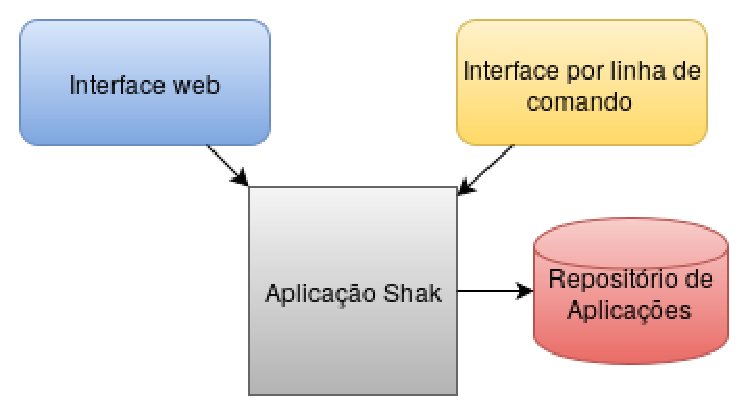
\includegraphics[width=0.5\textwidth]
      {figuras/shak}
      \caption{Arquitetura simplificada da ferramenta Shak}
  \label{fig:shak}
\end{figure}

No Shak, uma aplicação possui uma abstração que está exemplificada na figura \ref{fig:shak2},
onde uma aplicação é uma classe Ruby, e cada aplicação possui um livro de receitas
Chef associado. Além disso, cada livro de receitas pode definir quais são as entradas que
a aplicação necessita, como por exemplo, o endereço da aplicação. Essas entradas
são informadas, ou pela aplicação web, ou pela interface de linha de comando. As entradas 
também serão processadas pela aplicação Shak, que guarda essas informações no
seu repositório de aplicações. 

\begin{figure}[h]
  \centering
  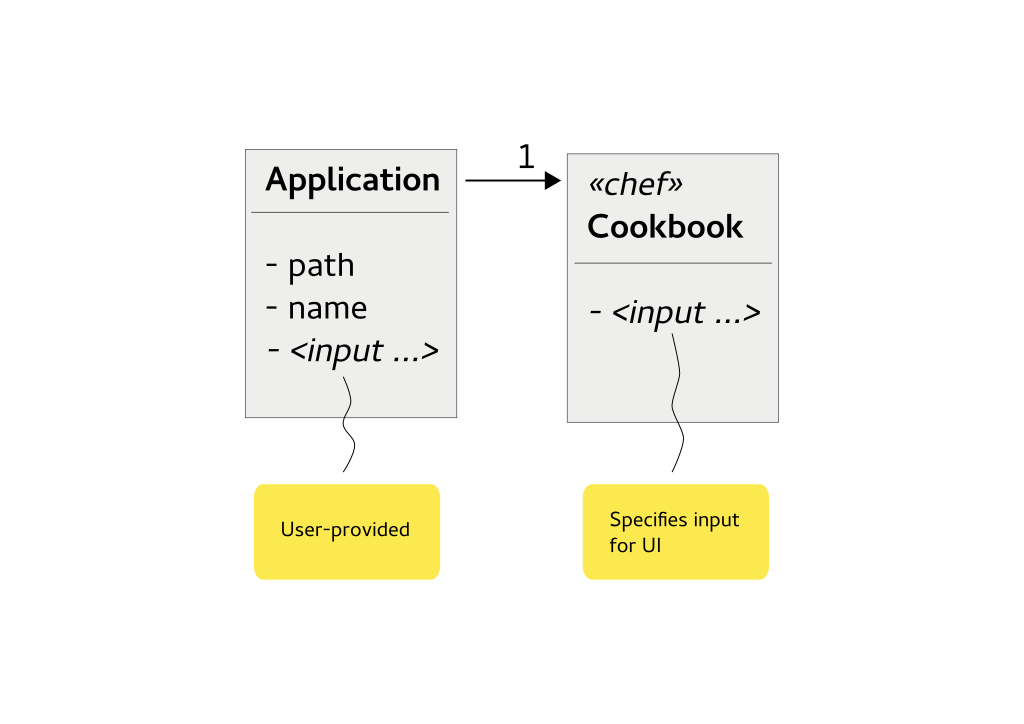
\includegraphics[width=0.7\textwidth]
      {figuras/data-model}
      \caption{Modelo de dados do Shak}
  \label{fig:shak2}
\end{figure}

Em resumo, a estrutura do Shak utiliza:

\begin{itemize}
  \item  \textbf{Livro de Receitas Chef:} Uso de livros de receitas
  para poder organizar a instalação de cada componente, contendo um livro
  de receitas para cada aplicação que for instalada.
  \item  \textbf{Código Ruby:} Arquitetura desenvolvida na linguagem
  Ruby, com programação orientado a objetos.
  \item  \textbf{Servidor web:} O servidor web é o Nginx, que é um
  servidor \textit{HTTP} de alto desempenho \cite{nginx}.
  \item  \textbf{Pacotes Debian:} As bibliotecas utilizadas estão incluídos na distribuição
  oficial do Debian.
  \item  \textbf{Gems:} Uso de gems para a aplicação,
  uma gem nada mais é do que uma biblioteca Ruby, que provê um formato padrão para
  a distribuição de programas Ruby \cite{gem}.
  \item  \textbf{Código Shellscript:} Os códigos ShellScript são utilizados
  principalmente para configurações de ambiente de desenvolvimento. 
\end{itemize}

Para adicionar uma aplicação que esteja disponível nos repositórios oficiais
do Debian na ferramenta Shak, é necessário construir o seu respectivo 
livro de receitas, utilizando Chef. 

Para adicionar uma receita Chef à ferramenta Shak, existe um recurso no Shak que
automatiza todo esse processo, no qual cria uma estrutura padrão de livro de receitas
Chef. Para usar esse recurso, é necessário executar o comando \textit{rake cookbook}
no terminal, além de informar o nome do livro de receitas desejado. O resultado
disso é a criação de arquivos e pastas, que formam a estrutura de um livro de receitas. Um
exemplo disso é o livro de receitas da aplicação MoinMoin, como na figura \ref{fig:x}. 

\begin{figure}[H]
  \centering
  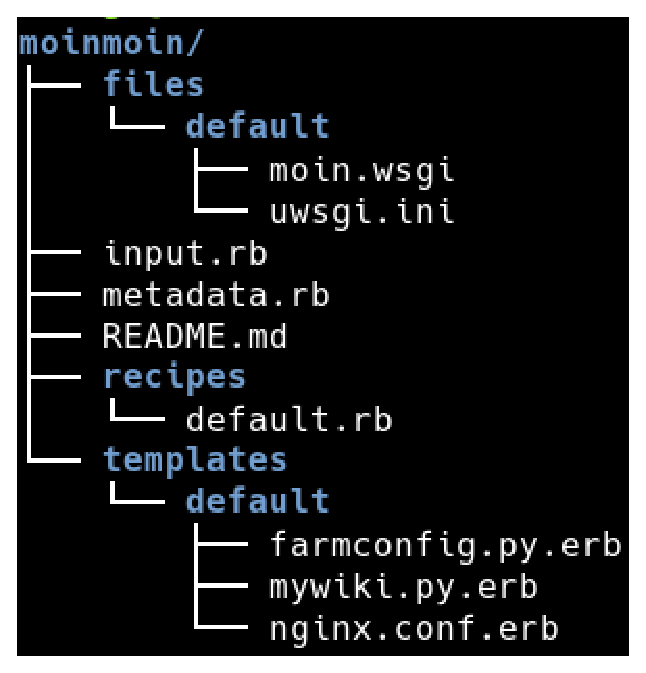
\includegraphics[width=0.5\textwidth]
      {figuras/cookbook}
      \caption{Estrutura do livro de receitas no Shak.}
  \label{fig:x}
\end{figure}

As receitas ficam no diretório \textit{recipes}, o Shak sempre executa a receita que está
no arquivo \textit{default.rb}, mas isso não impede a criação de outras receitas em outros arquivos,
desde que sejam incluídas nesse arquivo. 

Os arquivos de configuração ficam nos diretórios \textit{files} e \textit{templates},
a diferença entre eles é que no diretório \textit{files} ficam os arquivos que
não são alterados, ou seja, esses arquivos não vão precisar de alterações
durante a implantação. 

Já no diretório \textit{templates}, ficam os arquivos de configuração que sofrem alterações durante 
a implantação. Além disso, os arquivos template possuem uma característica, eles 
são arquivos no formato .erb \textit{(Embedded Ruby)}, que permite que o 
implantador adicione código Ruby no arquivo de texto. Isso permite configurações
mais robustas, durante a implantação da aplicação.

Também existem os arquivos que estão na raiz do livro de receitas. O \textit{input.rb}
é o arquivo em que é possível declarar os atributos das aplicações. Também é 
possível declarar quais atributos são obrigatórios e quais são únicos.

O código \ref{codigox} possui um exemplo de arquivo \textit{input.rb}.

\begin{lstlisting}[basicstyle=\ttfamily, language=Ruby,label=dice_index,caption={Exemplo de código no arquivo input.rb}, label=codigox]
text :hostname do
  title 'Website domain'                                                        
  mandatory                                                                     
end                                                                             
                                                                                
text :path do                                                                   
  title 'Path'                                                                  
  default '/'                                                                   
end                                                                             
                                                                                
unique :hostname, :path 
\end{lstlisting}

Por fim, os arquivos \textit{metadata.rb} e \textit{README.md}, o primeiro possui
informações sobre o livro de receitas, como o nome, o mantenedor do livro
de receitas, e sua licença. Já o segundo, possui instruções para utilizar a 
receita.

Com a estrutura criada, foi necessário construir as receitas, para automatizar
a implantação das aplicações. A atividade de 
criação de receitas e suporte das aplicações foi uma das atividades 
deste trabalho, sendo assim, adicionando novas aplicações web à ferramenta Shak.

\subsection{Gerência de Ambientes de Desenvolvimento}

Uma das necessidades do desenvolvimento do projeto é ter um ambiente de desenvolvimento
flexível, que possa ser rapidamente construído e destruído. Onde seja possível 
testar as implantações feitas pela ferramenta Shak e verificar os erros da implantação, caso 
aconteçam. 

Para isso, foi necessário utilizar alguma ferramenta que automatize o processo de 
construir ambientes de desenvolvimento. Construir ambientes manualmente pode
ser um processo longo e demorado, além disso, é possível que ocorra erros por
desatenção ao executar vários passos manuais. A ferramenta escolhida serviu para
auxiliar na criação das máquinas virtuais, que eram os nós alvo 
das implantações.

A ferramenta que foi escolhida para auxiliar na gerência de um ambiente de desenvolvimento é
a ferramenta Vagrant \footnote{https://www.vagrantup.com/}. Com o Vagrant é 
possível gerenciar a criação de máquinas
virtuais para os ambientes de desenvolvimento do projeto.

O ambiente de desenvolvimento escolhido, foi um ambiente com o sistema Debian na sua versão
sid 64 bits(que é a versão que contém os pacotes mais atuais, conhecida como versão instável),
apesar de a versão ser a versão instável, isso foi importante para que tenha disponível 
as versões mais novas dos pacotes das ferramentas escolhidas. Além disso, é preciso que a ferramenta Shak suporte primeiramente a versão instável do Debian, para que assim 
fosse incluída no próximo lançamento estável do Debian.

\section{Planejamento das Atividades}

As atividades planejadas para a evolução da ferramenta Shak são baseadas nas 
aplicações que foram escolhidas na Seção
\ref{subsection:exemplos}. Essas foram as aplicações que tiveram
sua implantação automatizadas pela ferramenta. 

No trabalho, foi feito uma fase exploratória, no qual o planejamento foi
suportar a instalação do Owncloud e Wordpress de forma 
automatizada. A escolha das duas ferramentas foi feita pelo autor e pelo co-orientador
deste trabalho, levando em consideração a popularidade das duas ferramentas nas 
comunidades de software livre. 

Essa fase exploratória foi necessária para evoluir a ferramenta
, visto que a ferramenta Shak só suportava aplicações estáticas, ou seja, apenas 
aplicações que contenham 
código \textit{HTML}, \textit{CSS} e \textit{Javascript}. 

A fase exploratória foi importante para apoiar na definição das fases e 
procedimentos para implantação
automatizada. Além de que, a partir dela, foram definidas características importantes 
que devem ser levadas em consideração para a escolha das próximas aplicações.

As atividades levantadas foram:

 \begin{enumerate}
   \item  Suporte a instalação automatizada do Wordpress.
   \item  Suporte a instalação automatizada do Owncloud.
   \item  Forçar as aplicações Wordpress e Owncloud a
   utilizar o protocolo HTTPS.
   \item  Suporte a instalação automatizada do servidor de e-mail.
   \item  Suporte a instalação automatizada do MoinMoin.
   \item  Suporte a instalação automatizada do Roundcube.
   \item  Suporte a instalação automatizada do Noosfero.
 \end{enumerate}

Ao verificar que tanto a ferramenta Owncloud como a ferramenta Wordpress precisam
de configurações de servidor de e-mail para algumas funcionalidades, também foi adicionado
a atividade de criação de uma receita para a automatizar a configuração de
servidor de e-mail. Como aspecto de segurança, ficou definido que tanto a aplicação
Owncloud como Wordpress deveriam usar sempre HTTPS por padrão, isso envolve também
uma estratégia de como serão gerenciados os certificados de segurança para aplicar
o protocolo HTTPS. 

Após a fase exploratória, outras aplicações foram escolhidas, são elas o MoinMoin, 
Roundcube e Noosfero, de acordo com as características desejadas, 
definidas na Seção \ref{subsection:validacao}

Dentro da implantação automatizada de software Debian GNU/Linux, existem várias
configurações possíveis. Neste trabalho, existem algumas características que foram 
levadas em consideração, são elas:

\begin{enumerate}
  \item  Segurança na implantação de aplicações web,
   como por exemplo utilizar protocolos como \textit{HTTPS}.
  \item  Configuração de múltiplas instâncias de
   aplicações, utilizando hospedagem virtual.
\end{enumerate}

Por fim, foi necessário definir procedimentos para a execução da implantação 
automatizada das aplicações. Considerando
o processo de implantação de software visto no Capítulo \ref{cap-referencial}
e a referência dos trabalhos relacionados. Foi necessário definir as fases e os
procedimentos para implantação automatizada, definindo as etapas
da implantação.

\subsection{Fases e Procedimentos para implantação}
\label{sec:fases}

Primeiramente, era necessária a definição das fases e os procedimentos para a implantação 
automatizada, de acordo com as fases que compõem o processo de 
implantação de aplicações, e de acordo com a Subseção \ref{sub:processoimplantacao}. 

Neste trabalho, foi adicionado na fase de configuração, a atividade de configuração de múltiplas
instâncias, que é a fase responsável por habilitar a implantação de múltiplas 
instâncias de uma aplicação. Isso possibilita a configuração de várias instâncias da mesma aplicação sem duplicação de recursos. A sequência
das fases estão na figura \ref{fig:1}:

\begin{figure}[h]
  \centering
  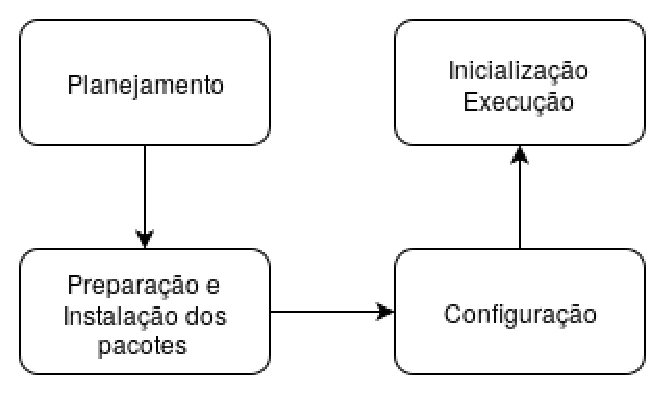
\includegraphics[width=0.8\textwidth]
      {figuras/fases}
      \caption{Sequência de fases para implantação automatizada de aplicações}
  \label{fig:1}
\end{figure}

\begin{enumerate}
  \item  \textbf{Planejamento}: Identificar os componentes mínimos necessários na implantação
 da aplicação.  
  \item  \textbf{Preparação e Instalação de Pacotes}: Preparar o ambiente alvo, 
isso envolve configuração do sistema operacional e instalação de dependências necessárias.
  \item  \textbf{Configuração}: Editar os arquivos de configuração necessários, tanto 
da aplicação como de suas dependências. Além disso, configurar o suporte de múltiplas instâncias
da aplicação.   
  \item  \textbf{Inicialização/Execução}: Testar as receitas construídas, utilizando
a ferramenta Shak. 
\end{enumerate}

Também foram definidas as caraterísticas de segurança que as aplicações devem 
ter na  sua implantação, foi 
definido que as aplicações sempre usem protocolos 
seguros, como o \textit{HTTPS}. 
Para as aplicações web é necessário utilizar o protocolo HTTPS, para aplicações
de e-mail é necessário utilizar os protocolos \textit{SMTP} e \textit{IMAPS}.

\subsection{Validação da solução}
\label{subsection:validacao}

Para validar a evolução da ferramenta, foram feitos exemplos de uso,
com as aplicações definidas, ou seja, aplicações que tenham todo o seu 
processo de instalação e configuração automatizado, a
fim de refinar e evoluir a ferramenta, conforme problemas forem surgindo. A escolha
desses exemplos de uso devem ser feitas a partir de aplicações reais e
conhecidas na comunidade de software livre. 

Depois da fase exploratória, observam-se outras características importantes, e que 
devem ser levados em consideração para a escolha das aplicações, além da 
popularidade, utilizado anteriormente. As seguintes 
características foram levadas em consideração para a escolha das aplicações:

\begin{description}
  \item  [Aplicações empacotadas no Debian:] Como o intuito do trabalho
  é realizar implantações múltiplas a partir de um pacote único, tais aplicações
  devem estar empacotadas e disponíveis para instalação nos servidores do Debian. Caso
a aplicação não esteja disponível no Debian, é necessário empacotá-la e distribuir
nos servidores oficiais do Debian.
 \item  [Servidor web compatível:] As ferramentas escolhidas possuem, no
  mínimo, o servidor web compatível. Por exemplo, todas as aplicações devem 
possuir suporte ao servidor Nginx ou Apache.
  \item  [Aplicações com comunidades ativas:] É importante que os softwares 
escolhidos possuam comunidades ativas, isso pode ajudar na resolução de possíveis 
problemas. Logo, aplicações abandonadas pela sua comunidade foram evitadas, e
  aplicações com comunidade de desenvolvedores e usuários ativas foram priorizadas.
  Por utilizar a distribuição instável, é possível que sejam descobertos
  erros na integração dessas ferramentas com o Debian. Tais erros e melhorias são
  reportados para o Debian, ou até solucionados, e 
  devolvidos aos mantenedores dos pacotes.
  \item  [Documentação do software:] A documentação do software também foi
  levada em consideração, principalmente a documentação da instalação e configuração
  dentro da ferramenta. As ferramentas que não possuem documentação de instalação e
  configuração foram evitadas.
  \item  [Aplicações com suporte a federação:] Aplicações federadas permitem
 utilização de métodos de autenticação única para cada instância da aplicação,
mantendo a compatibilidade entre elas, um exemplo é a aplicação Owncloud,
que permite compartilhar seus arquivos na nuvem independente do Owncloud que estiver usando,
isto é possível utilizando apenas um identificador único, chamado ID Federated Cloud, assim
possibilitando que os arquivos do usuário sejam compartilhados entre suas instâncias do
Owncloud na nuvem.
\end{description}

A partir dessas características definidas, também era necessário encontrar os exemplos de uso
utilizados para a execução da solução.

\subsection{Exemplos de uso: busca dos pacotes das aplicações}
\label{subsection:exemplos}

Para encontrar as aplicações que possam se encaixar dentro desses parâmetros foi necessário buscar por alguns exemplos de uso. Para a escolha das aplicações que
foram utilizadas como exemplos de uso, foi necessário fazer uma busca nas aplicações
web  que possuem suporte a configuração de múltiplas
instâncias, essa busca levou em consideração também, a documentação para realizar
tal configuração. Foram levantados algumas aplicações web da seguinte forma:

\begin{center}
apt-cache search web | wc -l
\end{center}

O resultado obtido com pacotes que contenham a palavra web recebe o resultado de 3470
pacotes de diversas aplicações ou módulos de aplicações, como
Wordpress; Owncloud; Drupal; Mailman e Chromium.
 
Foram escolhidas as aplicações Wordpress, Owncloud, MoinMoin
e Roundcube, por conter as características definidas anteriormente. Além disso,
também foi escolhida a aplicação Noosfero, que é uma aplicação que ainda não
está no Debian, porém neste trabalho será feito um esforço inicial para que isso
seja possível.

Para realizar a implantação das aplicações, foi importante que as 
instalações e configurações
fossem executadas num ambiente limpo. Os testes foram criados
em máquinas virtuais com a configuração conhecida como mínima, que contém
instalado apenas as aplicações necessárias para o funcionamento do sistema operacional.

Após a execução da implantação, o testador verificou o perfeito
funcionamento de algumas funcionalidades básicas das aplicações escolhidas,
e principalmente verificar a implantação de várias instâncias da mesma
aplicação no mesmo servidor destino, observando o perfeito funcionamento de todas as
instâncias implantadas, para assim, validar a implantação de múltiplas instâncias, conforme
apresentado nos resultados do próximo capítulo.
